En el segundo sprint se describe el procedimiento llevado a cabo para el uso de los estados meteorológicos obtenidos de la API de AEMET~\cite{Aemet}.

Tal y como se comentó en el sprint anterior, la respuesta a la petición \textit{requests} recibida por dicha API consta de estados meteorológicos en formato de cadena de texto. Un ejemplo de respuesta se muestra (simplificado) en el listado 4.3. (\textcopyright AEMET)

\begin{lstlisting}[numbers=none,caption={Ejemplo de respuesta de la API - AEMET}]]
{
 origen: {
	productor: "Agencia Estatal de Meteorología - AEMET. Gobierno de España",
	web: "http://www.aemet.es",
	language: "es",
	copyright: "AEMET. Autorizado el uso de la información y su reproducción citando a AEMET como autora de la misma.",
	notaLegal: "http://www.aemet.es/es/nota_legal"
 },
 elaborado: "2019-2-12",
 nombre: "Consuegra",
 provincia: "Toledo",
 prediccion: {
 	dia: [
		{
		 estadoCielo: [
					{
					 periodo: "08",
					 descripcion: "Cubierto"
					},
					{
					 periodo: "09",
					 descripcion: "Cubierto con lluvia escasa"
					},
					{
					 periodo: "10",
					 descripcion: "Cubierto con lluvia escasa"
					},
					{
					 periodo: "11",
					 descripcion: "Cubierto"
					},
					...
		 ]
		}
	}
}
\end{lstlisting}

Cómo se puede observar, en el campo 'predicción' existe un subcampo 'estadoCielo' (entre otros que se han obviado por no ser de interés en este trabajo) que contiene una lista con los estados meteorológicos. Cada elemento de la lista contiene dos valores: período (hora del día de esa previsión) y descripción (cadena de texto que describe el estado del cielo). Claramente existe un problema, ya que para la determinación de la máxima energía fotovoltaica posible en una hora determinada debe conocerse la potencia nominal posible (potencia que es capaz de suministrar el módulo fotovoltaico), directamente proporcional al estado meteorológico, el cuál es un texto que describe la situación y no un valor numérico que representa los watios que puede dar un módulo en esas condiciones, y a priori no se dispone de una forma directa de relacionarlas. \\

Se emplea \textbf{lógica difusa} para poder resolver la problemática mencionada anteriormente.
\subsection{Lógica difusa}
La teoría de la lógica difusa proporciona un marco matemático que permite modelar la incertidumbre de los procesos cognitivos humanos para poder ser tratable por un computador. Estos procesos cognitivos hacen referencia a expresiones del tipo:
\begin{itemize}
	\item Si no vives \textit{lejos} puedes ir en bicicleta. 
	\item Si hace \textit{mucho} frío llévate un chaquetón. 
\end{itemize} 
Los humanos son capaces de interpretar estos valores rápidamente, aunque no existe un valor cuantitativo que indique la distancia a la que se refiere la palabra \textit{lejos} o cuánto es \textit{mucho} frío. Sin embargo, las máquinas tienen algún que otro problema. Si se intentan trasladar estas reglar a código, aparecen dificultades ya que no se puede procesar numéricamente. Una opción es definir intervalos de valores que comprende cada palabra (por ejemplo, tomando \textit{lejos} como la distancia comprendida entre 5 y 10 kilómetros), pero esto no es preciso ya que para un computador, la distancia de 5,01 kilómetros sería lejos rotundamente, cuando en realidad la interpretación correcta no es así. Con ésto queda a la vista que la lógica convencional no trata de forma eficiente este problema. La solución pasa por emplear un método de razonamiento afín a la lógica difusa. \\

La lógica difusa permite representar matemáticamente la \textbf{incertidumbre}, mediante el empleo de herramientas formales. Según Zadeh~\cite{Zad73}, "\textit{Cuando aumenta la complejidad, los enunciados precisos pierden su significado y los enunciados útiles pierden precisión.}", es decir, \textit{los árboles no te dejan ver el bosque}, pues prácticamente cualquier problema del mundo puede resolverse partiendo de unas variables de entrada y buscando obtener como objetivo un conjunto de variables de salida. La lógica difusa establece esa relación entre variables de forma correcta.

\subsection{\textit{Fuzzy Sets}}



\begin{figure}[!h]
	\centering
	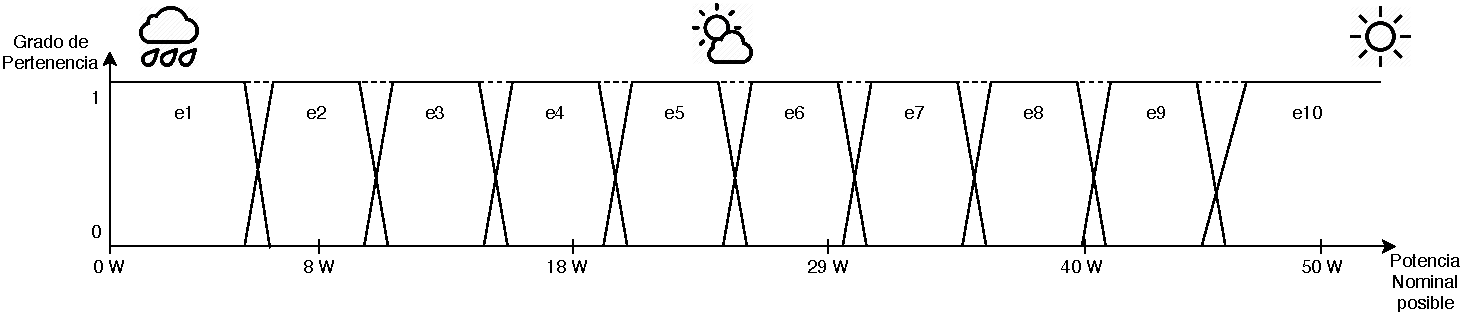
\includegraphics[width=17cm]{figs/Fuzzy_diagram.pdf}
	\caption{\textit{Fuzzy sets de los estados meteorológicos}}
\end{figure}